% Chapter Template

\chapter{Ensayos y resultados} % Main chapter title

\label{Chapter4} % Change X to a consecutive number; for referencing this chapter elsewhere, use \ref{ChapterX}

En este capítulo se detallan los ensayos y mediciones realizados sobre el sistema, para validar su funcionamiento y el cumplimiento de los requerimientos del trabajo. Se explicará cómo está compuesto el banco de pruebas utilizado y los instrumentos empleados, cómo se comprobó el envío de mensajes CAN a través de la red, qué ensayos eléctricos se realizaron sobre el sistema y cómo se verificó el envío de datos a través de UART y USB. Finalmente, se hablará de los ensayos que se realizaron en la planta de Cambre ICyFSA. 

%----------------------------------------------------------------------------------------
%	SECTION 1
%----------------------------------------------------------------------------------------

\section{Banco de pruebas}

Para validar el correcto funcionamiento del sistema, se ensambló un conjunto, se le cargó el firmware y se armó una red CAN con algunos motores paso a paso con plaquetas SN-17 conectadas. Dependiendo el ensayo a realizar, se conectaron 1 o más motores a la red, junto con un osciloscopio INSERTAR MARCA DEL OSCILOSCOPIO). Los dispositivos se alimentan con una fuente DC regulable YIHUA 305D\footnote{\url{http://yihuasoldering.com/product-4-2-30v-dc-power-supply/160008/}} trabajando a 24 V.

En la Figura \ref{fig:Banco} puede verse un esquema de la composición del banco de pruebas y los conexionados. En la PC se corre un programa de monitor serial llamado PuTTy\footnote{\url{https://www.putty.org/}} que se emplea para visualizar de forma simplificada el mensaje que el sistema intenta envíar a la red CAN.

\begin{figure}[htbp]
	\centering
	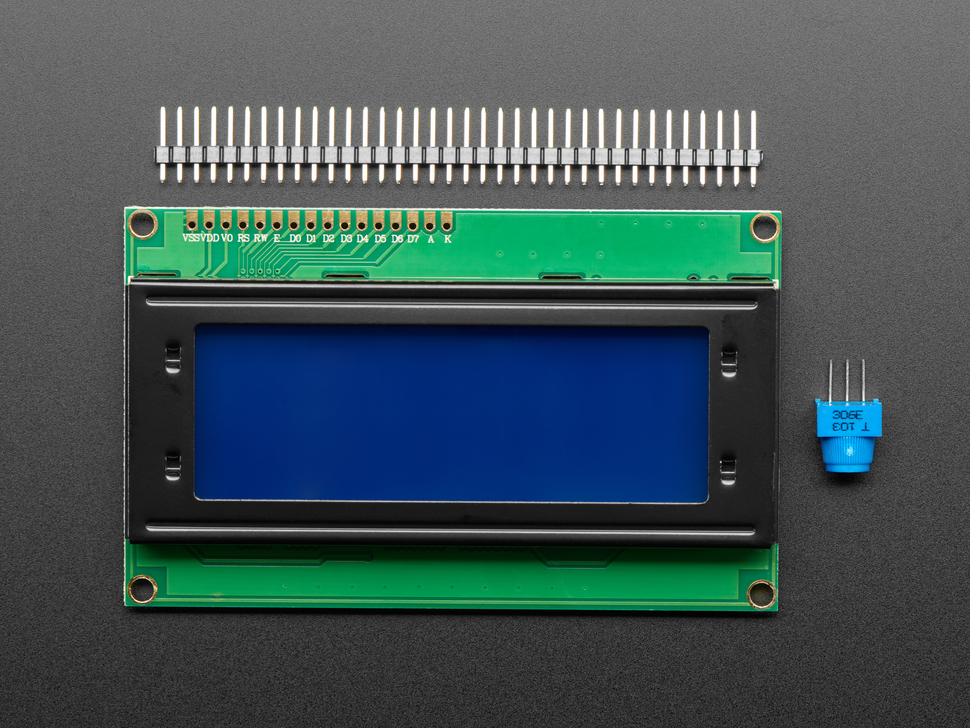
\includegraphics[scale=1]{./Figures/LCD.jpg}
	\caption{Banco de pruebas utilizado para verificaciones}
	\label{fig:Banco}
\end{figure}



\section{Ensayo de mensajes CAN}

En la Figura \ref{fig:niv_señal} se puede ver una de las tramas CAN tomadas desde el osciloscopio. En esta, se pueden ver claramente las señales CAN-H y CAN-L en un estado recesivo a 2.5 V y separándose un poco más de 1 V en ambos sentidos en un estado dominante, este es el comportamiento esperado. Notar también la falta de ruido en la señal, lo que indica la correcta operación de los resistores de terminación

\begin{figure}[htbp]
	\centering
	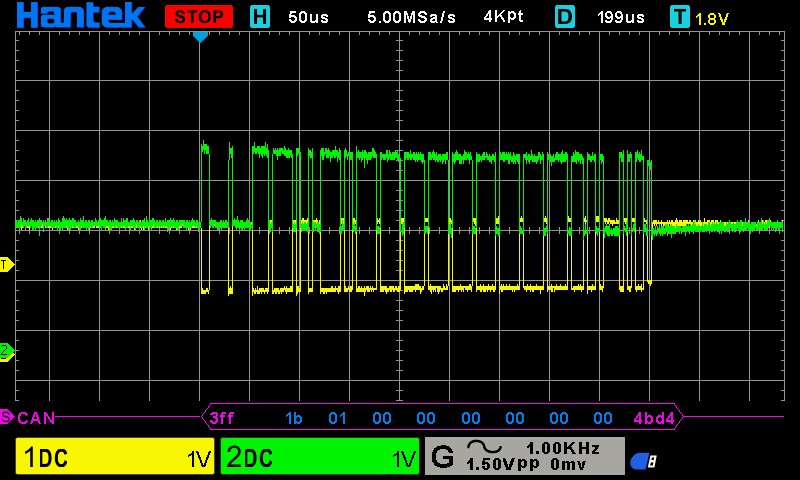
\includegraphics[scale=0.6]{./Figures/Message_Change_Operation_Mode_CONFIG.jpg}
	\caption{Níveles de señal CAN en osciloscopio}
	\label{fig:niv_señal}
\end{figure}

AGREGAR MEDICION DE TIEMPO

Para la verificación de los mensajes CAN se probaron cada uno de los mensajes posibles. Se revisó que el identificador y la data fueran correctas y que los sistemas conectados realizaran las acciones correspondientes.

En la Figura \ref{fig:mot_calib} se puede ver una imagen tomada del osciloscopio para la instrucción de calibrar motor (código: 0x0c). En la parte iferior puede verse el decodificador CAN que el osciloscopio trae incorporado, marcando correctamente la instrucción. También, se puede ver el identificador del mensaje (código: 0x0b) compuesto por el identificador del motor (0x05) y el bit final indicando que es un mensaje desde el dispositivo controlador. El resto de los bytes de data se marcan en 0, ya que no es necesario envíar más información para este tipo de mensaje, los últimos bytes pertenecen al CRC.

\begin{figure}[htbp]
	\centering
	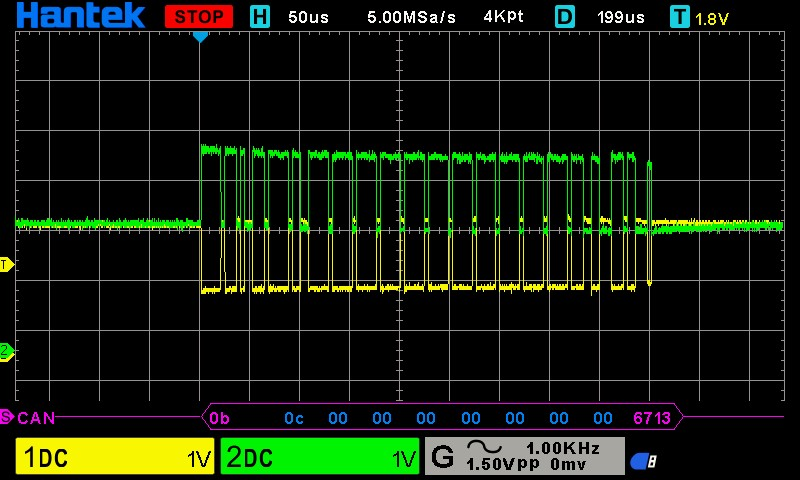
\includegraphics[scale=0.6]{./Figures/Motor_Calibrate.jpg}
	\caption{Instrucción calibrar motor}
	\label{fig:mot_calib}
\end{figure}

Otro ejemplo de mensaje puede visualizarse en la Figura \ref{fig:mot_move} en la que se envía al motor un comando manual de movimiento angular (código: 0x10), en dirección en contra de las agujas del reloj (código 0x01), un ángulo de 360 grados (códigos: 0x01 y 0x68). En este caso, como este ángulo es un número que requiere más de un byte para su representación, aparece descompuesto en el mensaje. Si se hace la conversión del número 168, de hexadecimal a decimal, se comprueba que es efectivamente 360. Al recibir el mensaje, el motor correctamente gira lo estipulado.

\begin{figure}[htbp]
	\centering
	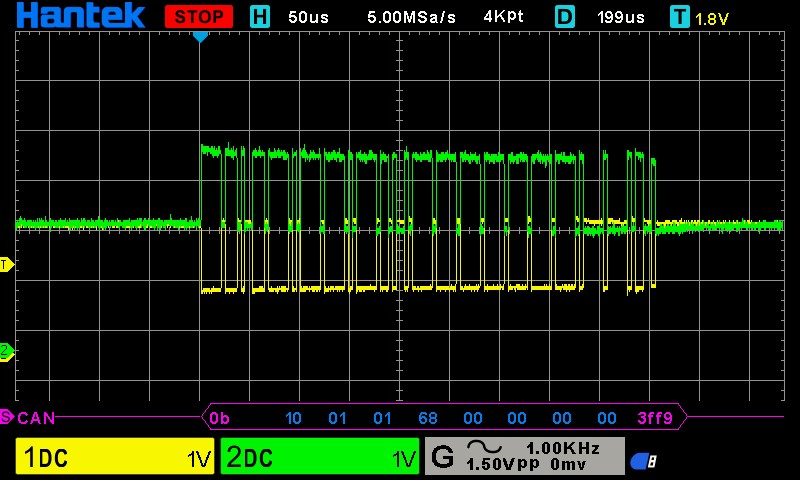
\includegraphics[scale=0.6]{./Figures/Motor_Manual_Move_CCW_360DEG.jpg}
	\caption{Instrucción manual mover motor}
	\label{fig:mot_move}
\end{figure}

\section{Ensayos eléctricos}

\section{Ensayos de mensajes UART}

\section{Pruebas de funcionamiento en planta}

\section{Comparación con estado del arte}
